% ============================================================
% CHAPTER 3: Sprint 3 & Sprint 4 — Users, Dashboard, VM Management
% ============================================================
% ADD THIS TO main.tex AFTER COMPLETING SPRINT 3 & 4
% Uncomment: % ============================================================
% CHAPTER 3: Sprint 3 & Sprint 4 — Users, Dashboard, VM Management
% ============================================================
% ADD THIS TO main.tex AFTER COMPLETING SPRINT 3 & 4
% Uncomment: % ============================================================
% CHAPTER 3: Sprint 3 & Sprint 4 — Users, Dashboard, VM Management
% ============================================================
% ADD THIS TO main.tex AFTER COMPLETING SPRINT 3 & 4
% Uncomment: % ============================================================
% CHAPTER 3: Sprint 3 & Sprint 4 — Users, Dashboard, VM Management
% ============================================================
% ADD THIS TO main.tex AFTER COMPLETING SPRINT 3 & 4
% Uncomment: \input{chapters/chapter3}
% ============================================================
\chapter{Sprint 3 \& Sprint 4: User Management and VM Operations}

\section{Introduction}

This chapter covers the core features of the platform. Sprint 3 implements user management, the dashboard layout, and NATS JetStream integration. Sprint 4 delivers the central feature — virtual machine lifecycle management through the VM service, Python worker, and OpenNebula integration.

% ============================================================
% SPRINT 3
% ============================================================
\section{Sprint 3: User Management \& Dashboard}

\sprintcard{3}{User Management \& Dashboard}{Implement user CRUD, admin management panel, dashboard layout, and message queue setup.}

\subsection{Sprint Backlog}

\begin{longtable}{|c|p{5cm}|c|c|c|}
\hline
\rowcolor{blue!15}
\textbf{Task ID} & \textbf{Task} & \textbf{Assignee} & \textbf{Est.} & \textbf{Status} \\
\hline
\endhead
T-3.1 & User service CRUD endpoints & DSI & 4h & Done \\
\hline
T-3.2 & Admin user management endpoints & DSI & 3h & Done \\
\hline
T-3.3 & Dashboard layout (sidebar, header) & DSI & 6h & Done \\
\hline
T-3.4 & Profile page (view/edit) & DSI & 4h & Done \\
\hline
T-3.11 & SSH key management (CRUD + UI) & DSI & 5h & Done \\
\hline
T-3.5 & Admin — user list page & DSI & 4h & Done \\
\hline
T-3.6 & NATS JetStream setup & DSI & 4h & Done \\
\hline
T-3.7 & Firewall rules (iptables) & RSI & 6h & Done \\
\hline
T-3.8 & Firewall testing & RSI & 4h & Done \\
\hline
T-3.9 & OpenNebula API access & RSI & 6h & Done \\
\hline
\caption{Sprint 3 backlog}
\label{tab:sprint3-backlog}
\end{longtable}

\subsection{Use Case Diagram — User Management}

\begin{figure}[H]
\centering
\begin{tikzpicture}[
  usecase/.style={draw, ellipse, minimum width=3cm, minimum height=0.8cm, align=center, font=\scriptsize}
]
  % System boundary
  \draw[thick, rounded corners] (0, -6.5) rectangle (6, 0.5);
  \node[font=\small\bfseries] at (3, 0.2) {User Management Module};
  
  % Actors
  \node (user) at (-2, -1.5) {User};
  \node (admin) at (-2, -5) {Admin};
  
  % Use cases
  \node[usecase] (uc1) at (3, -0.5) {View Profile};
  \node[usecase] (uc2) at (3, -1.5) {Edit Profile};
  \node[usecase] (uc3) at (3, -2.5) {Change Password};
  \node[usecase] (uc6) at (3, -3.5) {Manage SSH Keys};
  \node[usecase] (uc4) at (3, -4.5) {View All Users};
  \node[usecase] (uc5) at (3, -5.5) {Delete/Ban User};
  
  % Arrows
  \draw (user) -- (uc1);
  \draw (user) -- (uc2);
  \draw (user) -- (uc3);
  \draw (user) -- (uc6);
  \draw (admin) -- (uc4);
  \draw (admin) -- (uc5);
  
  % Generalization
  \draw[->, dashed] (admin) -- (user);
  
\end{tikzpicture}
\caption{Use case diagram — User management}
\label{fig:uc-user}
\end{figure}

\subsection{Sequence Diagram — Admin Deletes User}

\begin{figure}[H]
\centering
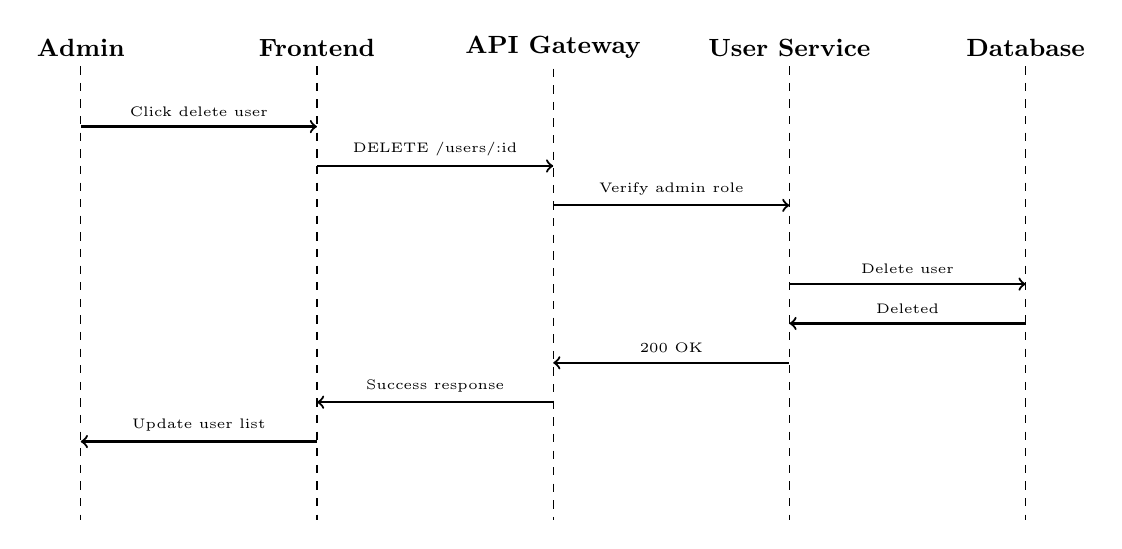
\begin{tikzpicture}[font=\small]
  \node (admin) at (0, 0) {\textbf{Admin}};
  \node (front) at (3, 0) {\textbf{Frontend}};
  \node (gate) at (6, 0) {\textbf{API Gateway}};
  \node (usvc) at (9, 0) {\textbf{User Service}};
  \node (db) at (12, 0) {\textbf{Database}};
  
  \draw[dashed] (admin) -- (0, -6);
  \draw[dashed] (front) -- (3, -6);
  \draw[dashed] (gate) -- (6, -6);
  \draw[dashed] (usvc) -- (9, -6);
  \draw[dashed] (db) -- (12, -6);
  
  \draw[->, thick] (0, -1) -- node[above, font=\tiny] {Click delete user} (3, -1);
  \draw[->, thick] (3, -1.5) -- node[above, font=\tiny] {DELETE /users/:id} (6, -1.5);
  \draw[->, thick] (6, -2) -- node[above, font=\tiny] {Verify admin role} (9, -2);
  \draw[->, thick] (9, -3) -- node[above, font=\tiny] {Delete user} (12, -3);
  \draw[<-, thick] (9, -3.5) -- node[above, font=\tiny] {Deleted} (12, -3.5);
  \draw[<-, thick] (6, -4) -- node[above, font=\tiny] {200 OK} (9, -4);
  \draw[<-, thick] (3, -4.5) -- node[above, font=\tiny] {Success response} (6, -4.5);
  \draw[<-, thick] (0, -5) -- node[above, font=\tiny] {Update user list} (3, -5);
\end{tikzpicture}
\caption{Sequence diagram — Admin deletes user}
\label{fig:seq-delete-user}
\end{figure}

\subsection{Implementation Screenshots}

\begin{figure}[H]
\centering
\fbox{\parbox{0.9\textwidth}{\centering\vspace{3cm}\textit{Insert dashboard layout screenshot}\vspace{3cm}}}
\caption{Dashboard layout with sidebar navigation}
\label{fig:dashboard-layout}
\end{figure}

\begin{figure}[H]
\centering
\fbox{\parbox{0.9\textwidth}{\centering\vspace{3cm}\textit{Insert admin user management screenshot}\vspace{3cm}}}
\caption{Admin — User management page}
\label{fig:admin-users}
\end{figure}

\begin{figure}[H]
\centering
\fbox{\parbox{0.9\textwidth}{\centering\vspace{3cm}\textit{Insert SSH key management page screenshot}\vspace{3cm}}}
\caption{SSH key management — User profile}
\label{fig:ssh-keys}
\end{figure}

\subsection{Sprint 3 Review}

At the end of Sprint 3:
\begin{itemize}
  \item User service with full CRUD operations.
  \item Admin panel for user management.
  \item Dashboard layout with sidebar, header, and responsive design.
  \item Profile page with edit functionality.
  \item SSH key management — users can add, view, and delete SSH public keys.
  \item NATS JetStream configured and tested.
  \item Firewall rules implemented and tested.
  \item OpenNebula XML-RPC API accessible and secured.
\end{itemize}


% ============================================================
% SPRINT 4
% ============================================================
\section{Sprint 4: VM Management \& Worker Service}

\sprintcard{4}{VM Management \& Worker Service}{Implement the core VM lifecycle operations — create, start, stop, reboot, delete — through the web platform with asynchronous processing via the Python worker.}

\subsection{Sprint Backlog}

\begin{longtable}{|c|p{5cm}|c|c|c|}
\hline
\rowcolor{blue!15}
\textbf{Task ID} & \textbf{Task} & \textbf{Assignee} & \textbf{Est.} & \textbf{Status} \\
\hline
\endhead
T-4.1 & VM service — Create VM endpoint & DSI & 5h & Done \\
\hline
T-4.2 & Python worker setup (Redis + NATS) & DSI & 5h & Done \\
\hline
T-4.3 & Worker — Create VM via OpenNebula & DSI & 5h & Done \\
\hline
T-4.4 & Worker — Start/Stop/Reboot ops & DSI & 4h & Done \\
\hline
T-4.5 & Worker — Delete VM operation & DSI & 2h & Done \\
\hline
T-4.6 & VM creation form (frontend) & DSI & 5h & Done \\
\hline
T-4.7 & VM list page (frontend) & DSI & 4h & Done \\
\hline
T-4.8 & OpenNebula API integration testing & RSI & 6h & Done \\
\hline
T-4.9 & VM networking (virtual networks) & RSI & 6h & Done \\
\hline
T-4.10 & Storage + disk images & RSI & 4h & Done \\
\hline
\caption{Sprint 4 backlog}
\label{tab:sprint4-backlog}
\end{longtable}

\subsection{Use Case Diagram — VM Management}

\begin{figure}[H]
\centering
\begin{tikzpicture}[
  usecase/.style={draw, ellipse, minimum width=2.8cm, minimum height=0.8cm, align=center, font=\scriptsize}
]
  % System boundary
  \draw[thick, rounded corners] (0, -7) rectangle (6.5, 0.5);
  \node[font=\small\bfseries] at (3.25, 0.2) {VM Management Module};
  
  % Actors
  \node (user) at (-2, -2) {User};
  \node (admin) at (9, -3) {Admin};
  
  % Use cases
  \node[usecase] (uc1) at (3.25, -0.5) {Create VM};
  \node[usecase] (uc2) at (3.25, -1.5) {Start VM};
  \node[usecase] (uc3) at (3.25, -2.5) {Stop VM};
  \node[usecase] (uc4) at (3.25, -3.5) {Reboot VM};
  \node[usecase] (uc5) at (3.25, -4.5) {Delete VM};
  \node[usecase] (uc6) at (3.25, -5.5) {View VM List};
  \node[usecase] (uc7) at (3.25, -6.5) {View VM Details};
  
  % Arrows
  \draw (user) -- (uc1);
  \draw (user) -- (uc2);
  \draw (user) -- (uc3);
  \draw (user) -- (uc4);
  \draw (user) -- (uc5);
  \draw (user) -- (uc6);
  \draw (user) -- (uc7);
  
  \draw (admin) -- (uc1);
  \draw (admin) -- (uc5);
  \draw (admin) -- (uc6);
  
\end{tikzpicture}
\caption{Use case diagram — VM management}
\label{fig:uc-vm}
\end{figure}

\subsection{Sequence Diagram — VM Creation (End-to-End)}

\begin{figure}[H]
\centering
\begin{tikzpicture}[font=\scriptsize]
  % Lifelines
  \node (user) at (0, 0) {\textbf{User}};
  \node (front) at (2, 0) {\textbf{Frontend}};
  \node (gate) at (4, 0) {\textbf{Gateway}};
  \node (vmsvc) at (6, 0) {\textbf{VM Service}};
  \node (nats) at (8, 0) {\textbf{JetStream}};
  \node (worker) at (10, 0) {\textbf{Worker}};
  \node (one) at (12.5, 0) {\textbf{OpenNebula}};
  
  \draw[dashed] (user) -- (0, -11);
  \draw[dashed] (front) -- (2, -11);
  \draw[dashed] (gate) -- (4, -11);
  \draw[dashed] (vmsvc) -- (6, -11);
  \draw[dashed] (nats) -- (8, -11);
  \draw[dashed] (worker) -- (10, -11);
  \draw[dashed] (one) -- (12.5, -11);
  
  % Messages
  \draw[->, thick] (0, -0.8) -- node[above] {Fill VM form} (2, -0.8);
  \draw[->, thick] (2, -1.5) -- node[above] {POST /vms} (4, -1.5);
  \draw[->, thick] (4, -2.2) -- node[above] {Forward} (6, -2.2);
  \draw[->, thick] (6, -2.7) -- node[right] {Check quota};
  \draw[->, thick] (6, -3.5) -- node[above] {Save VM (pending)} (6, -3.5);
  \draw[->, thick] (6, -4.2) -- node[above] {Publish event} (8, -4.2);
  \draw[<-, thick] (4, -4.9) -- node[above] {202 Accepted} (6, -4.9);
  \draw[<-, thick] (2, -5.3) -- node[above] {VM creating...} (4, -5.3);
  \draw[->, thick] (8, -6) -- node[above] {Consume event} (10, -6);
  \draw[->, thick] (10, -6.7) -- node[above] {Create VM} (12.5, -6.7);
  \draw[<-, thick] (10, -7.4) -- node[above] {VM ID + IP} (12.5, -7.4);
  \draw[->, thick] (10, -8.1) -- node[above] {Publish result} (8, -8.1);
  \draw[->, thick] (6, -8.8) -- node[above] {Update status} (6, -8.8);
  \draw[->, thick] (6, -9) -- node[right] {VM → running};
  \draw[<-, thick] (2, -9.7) -- node[above] {Status update} (6, -9.7);
  \draw[<-, thick] (0, -10.3) -- node[above] {VM ready!} (2, -10.3);
\end{tikzpicture}
\caption{Sequence diagram — VM creation (end-to-end)}
\label{fig:seq-vm-create}
\end{figure}

\subsection{Activity Diagram — VM Lifecycle}

\begin{figure}[H]
\centering
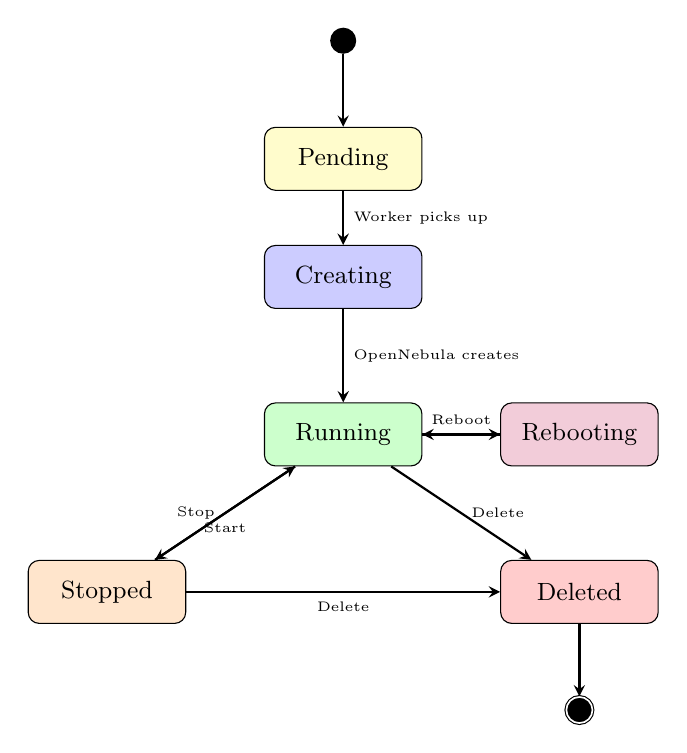
\begin{tikzpicture}[
  state/.style={draw, rounded corners, minimum width=2cm, minimum height=0.8cm, align=center, font=\small},
  decision/.style={draw, diamond, minimum width=1.5cm, minimum height=1cm, align=center, font=\tiny},
  arrow/.style={->, thick, >=stealth}
]
  % States
  \node[circle, fill=black, minimum size=0.3cm] (start) at (0, 0) {};
  \node[state, fill=yellow!20] (pending) at (0, -1.5) {Pending};
  \node[state, fill=blue!20] (creating) at (0, -3) {Creating};
  \node[state, fill=green!20] (running) at (0, -5) {Running};
  \node[state, fill=orange!20] (stopped) at (-3, -7) {Stopped};
  \node[state, fill=red!20] (deleted) at (3, -7) {Deleted};
  \node[state, fill=purple!20] (rebooting) at (3, -5) {Rebooting};
  \node[circle, draw, fill=black, minimum size=0.3cm, double] (end) at (3, -8.5) {};
  
  % Arrows
  \draw[arrow] (start) -- (pending);
  \draw[arrow] (pending) -- node[right, font=\tiny] {Worker picks up} (creating);
  \draw[arrow] (creating) -- node[right, font=\tiny] {OpenNebula creates} (running);
  \draw[arrow] (running) -- node[left, font=\tiny] {Stop} (stopped);
  \draw[arrow] (stopped) -- node[below, font=\tiny] {Start} (running);
  \draw[arrow] (running) -- node[above, font=\tiny] {Reboot} (rebooting);
  \draw[arrow] (rebooting) -- node[right, font=\tiny] {} (running);
  \draw[arrow] (running) -- node[right, font=\tiny] {Delete} (deleted);
  \draw[arrow] (stopped) -- node[below, font=\tiny] {Delete} (deleted);
  \draw[arrow] (deleted) -- (end);
\end{tikzpicture}
\caption{Activity diagram — VM lifecycle}
\label{fig:activity-vm}
\end{figure}

\subsection{Class Diagram — VM Module}

\begin{figure}[H]
\centering
\begin{tikzpicture}[font=\small,
  class/.style={draw, rectangle, minimum width=4cm, align=left}
]
  % VM class
  \node[class, fill=yellow!15] (vmclass) at (0, 0) {
    \textbf{VirtualMachine}\\
    \hline
    - id: UUID\\
    - name: String\\
    - userId: UUID\\
    - templateId: String\\
    - vcpu: Integer\\
    - ram: Integer (MB)\\
    - disk: Integer (GB)\\
    - status: VMStatus\\
    - ipAddress: String\\
    - oneId: Integer\\
    - createdAt: DateTime\\
    \hline
    + create()\\
    + start()\\
    + stop()\\
    + reboot()\\
    + delete()
  };
  
  % VMStatus enum
  \node[class, fill=green!15] (statusenum) at (6, 1) {
    \textbf{<<enum>> VMStatus}\\
    \hline
    PENDING\\
    CREATING\\
    RUNNING\\
    STOPPED\\
    REBOOTING\\
    DELETING\\
    DELETED\\
    ERROR
  };
  
  % VMTemplate
  \node[class, fill=blue!15] (template) at (6, -3.5) {
    \textbf{VMTemplate}\\
    \hline
    - id: String\\
    - name: String\\
    - os: String\\
    - minCpu: Integer\\
    - minRam: Integer\\
    - minDisk: Integer\\
    \hline
    + getTemplates()
  };
  
  % Relations
  \draw[->, thick] (vmclass) -- node[above, font=\tiny] {has} (statusenum);
  \draw[->, thick] (vmclass) -- node[below, font=\tiny] {uses} (template);
\end{tikzpicture}
\caption{Class diagram — VM module}
\label{fig:class-vm}
\end{figure}

\subsection{Architecture Diagram — Worker Communication}

\begin{figure}[H]
\centering
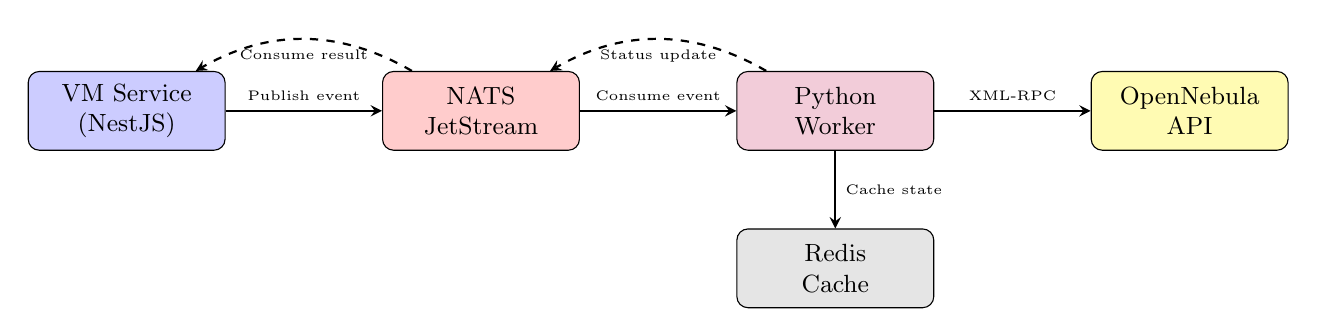
\begin{tikzpicture}[
  box/.style={draw, rounded corners, minimum width=2.5cm, minimum height=1cm, align=center, font=\small},
  arrow/.style={->, thick, >=stealth}
]
  \node[box, fill=blue!20] (vmsvc) at (0, 0) {VM Service\\(NestJS)};
  \node[box, fill=red!20] (nats) at (4.5, 0) {NATS\\JetStream};
  \node[box, fill=purple!20] (worker) at (9, 0) {Python\\Worker};
  \node[box, fill=gray!20] (redis) at (9, -2) {Redis\\Cache};
  \node[box, fill=yellow!30] (one) at (13.5, 0) {OpenNebula\\API};
  
  \draw[arrow] (vmsvc) -- node[above, font=\tiny] {Publish event} (nats);
  \draw[arrow] (nats) -- node[above, font=\tiny] {Consume event} (worker);
  \draw[arrow] (worker) -- node[above, font=\tiny] {XML-RPC} (one);
  \draw[arrow] (worker) -- node[right, font=\tiny] {Cache state} (redis);
  \draw[arrow, dashed] (worker) to[bend right=30] node[below, font=\tiny] {Status update} (nats);
  \draw[arrow, dashed] (nats) to[bend right=30] node[below, font=\tiny] {Consume result} (vmsvc);
\end{tikzpicture}
\caption{Architecture — Worker communication via JetStream}
\label{fig:worker-arch}
\end{figure}

\subsection{Implementation Screenshots}

\begin{figure}[H]
\centering
\fbox{\parbox{0.9\textwidth}{\centering\vspace{3cm}\textit{Insert VM creation form screenshot}\vspace{3cm}}}
\caption{VM creation form}
\label{fig:vm-create-form}
\end{figure}

\begin{figure}[H]
\centering
\fbox{\parbox{0.9\textwidth}{\centering\vspace{3cm}\textit{Insert VM list page screenshot}\vspace{3cm}}}
\caption{VM list page}
\label{fig:vm-list}
\end{figure}

\subsection{Sprint 4 Review}

At the end of Sprint 4:
\begin{itemize}
  \item VM service with full lifecycle operations (create, start, stop, reboot, delete).
  \item Python worker consuming events from NATS JetStream.
  \item Worker communicates with OpenNebula via XML-RPC API.
  \item VM creation form with template selection.
  \item VM list page with status indicators.
  \item OpenNebula virtual networks and storage configured.
  \item End-to-end VM creation working.
\end{itemize}

% ============================================================
\section{Conclusion}

In this chapter, we completed the user management features and the core VM operations. Sprint 3 delivered the admin panel, dashboard layout, and message queue infrastructure. Sprint 4 implemented the central feature of the platform — the ability to create and manage virtual machines through an asynchronous worker that communicates with OpenNebula.

In the next chapter, we will enhance the VM experience with a detailed dashboard, implement the quota system, and build the payment service.

% ============================================================
\chapter{Sprint 3 \& Sprint 4: User Management and VM Operations}

\section{Introduction}

This chapter covers the core features of the platform. Sprint 3 implements user management, the dashboard layout, and NATS JetStream integration. Sprint 4 delivers the central feature — virtual machine lifecycle management through the VM service, Python worker, and OpenNebula integration.

% ============================================================
% SPRINT 3
% ============================================================
\section{Sprint 3: User Management \& Dashboard}

\sprintcard{3}{User Management \& Dashboard}{Implement user CRUD, admin management panel, dashboard layout, and message queue setup.}

\subsection{Sprint Backlog}

\begin{longtable}{|c|p{5cm}|c|c|c|}
\hline
\rowcolor{blue!15}
\textbf{Task ID} & \textbf{Task} & \textbf{Assignee} & \textbf{Est.} & \textbf{Status} \\
\hline
\endhead
T-3.1 & User service CRUD endpoints & DSI & 4h & Done \\
\hline
T-3.2 & Admin user management endpoints & DSI & 3h & Done \\
\hline
T-3.3 & Dashboard layout (sidebar, header) & DSI & 6h & Done \\
\hline
T-3.4 & Profile page (view/edit) & DSI & 4h & Done \\
\hline
T-3.11 & SSH key management (CRUD + UI) & DSI & 5h & Done \\
\hline
T-3.5 & Admin — user list page & DSI & 4h & Done \\
\hline
T-3.6 & NATS JetStream setup & DSI & 4h & Done \\
\hline
T-3.7 & Firewall rules (iptables) & RSI & 6h & Done \\
\hline
T-3.8 & Firewall testing & RSI & 4h & Done \\
\hline
T-3.9 & OpenNebula API access & RSI & 6h & Done \\
\hline
\caption{Sprint 3 backlog}
\label{tab:sprint3-backlog}
\end{longtable}

\subsection{Use Case Diagram — User Management}

\begin{figure}[H]
\centering
\begin{tikzpicture}[
  usecase/.style={draw, ellipse, minimum width=3cm, minimum height=0.8cm, align=center, font=\scriptsize}
]
  % System boundary
  \draw[thick, rounded corners] (0, -6.5) rectangle (6, 0.5);
  \node[font=\small\bfseries] at (3, 0.2) {User Management Module};
  
  % Actors
  \node (user) at (-2, -1.5) {User};
  \node (admin) at (-2, -5) {Admin};
  
  % Use cases
  \node[usecase] (uc1) at (3, -0.5) {View Profile};
  \node[usecase] (uc2) at (3, -1.5) {Edit Profile};
  \node[usecase] (uc3) at (3, -2.5) {Change Password};
  \node[usecase] (uc6) at (3, -3.5) {Manage SSH Keys};
  \node[usecase] (uc4) at (3, -4.5) {View All Users};
  \node[usecase] (uc5) at (3, -5.5) {Delete/Ban User};
  
  % Arrows
  \draw (user) -- (uc1);
  \draw (user) -- (uc2);
  \draw (user) -- (uc3);
  \draw (user) -- (uc6);
  \draw (admin) -- (uc4);
  \draw (admin) -- (uc5);
  
  % Generalization
  \draw[->, dashed] (admin) -- (user);
  
\end{tikzpicture}
\caption{Use case diagram — User management}
\label{fig:uc-user}
\end{figure}

\subsection{Sequence Diagram — Admin Deletes User}

\begin{figure}[H]
\centering
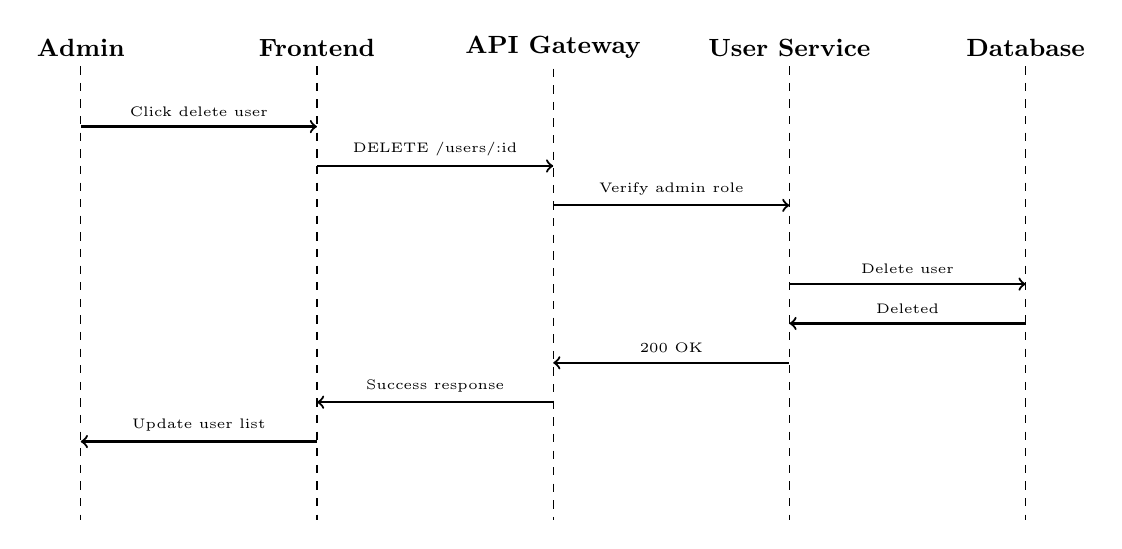
\begin{tikzpicture}[font=\small]
  \node (admin) at (0, 0) {\textbf{Admin}};
  \node (front) at (3, 0) {\textbf{Frontend}};
  \node (gate) at (6, 0) {\textbf{API Gateway}};
  \node (usvc) at (9, 0) {\textbf{User Service}};
  \node (db) at (12, 0) {\textbf{Database}};
  
  \draw[dashed] (admin) -- (0, -6);
  \draw[dashed] (front) -- (3, -6);
  \draw[dashed] (gate) -- (6, -6);
  \draw[dashed] (usvc) -- (9, -6);
  \draw[dashed] (db) -- (12, -6);
  
  \draw[->, thick] (0, -1) -- node[above, font=\tiny] {Click delete user} (3, -1);
  \draw[->, thick] (3, -1.5) -- node[above, font=\tiny] {DELETE /users/:id} (6, -1.5);
  \draw[->, thick] (6, -2) -- node[above, font=\tiny] {Verify admin role} (9, -2);
  \draw[->, thick] (9, -3) -- node[above, font=\tiny] {Delete user} (12, -3);
  \draw[<-, thick] (9, -3.5) -- node[above, font=\tiny] {Deleted} (12, -3.5);
  \draw[<-, thick] (6, -4) -- node[above, font=\tiny] {200 OK} (9, -4);
  \draw[<-, thick] (3, -4.5) -- node[above, font=\tiny] {Success response} (6, -4.5);
  \draw[<-, thick] (0, -5) -- node[above, font=\tiny] {Update user list} (3, -5);
\end{tikzpicture}
\caption{Sequence diagram — Admin deletes user}
\label{fig:seq-delete-user}
\end{figure}

\subsection{Implementation Screenshots}

\begin{figure}[H]
\centering
\fbox{\parbox{0.9\textwidth}{\centering\vspace{3cm}\textit{Insert dashboard layout screenshot}\vspace{3cm}}}
\caption{Dashboard layout with sidebar navigation}
\label{fig:dashboard-layout}
\end{figure}

\begin{figure}[H]
\centering
\fbox{\parbox{0.9\textwidth}{\centering\vspace{3cm}\textit{Insert admin user management screenshot}\vspace{3cm}}}
\caption{Admin — User management page}
\label{fig:admin-users}
\end{figure}

\begin{figure}[H]
\centering
\fbox{\parbox{0.9\textwidth}{\centering\vspace{3cm}\textit{Insert SSH key management page screenshot}\vspace{3cm}}}
\caption{SSH key management — User profile}
\label{fig:ssh-keys}
\end{figure}

\subsection{Sprint 3 Review}

At the end of Sprint 3:
\begin{itemize}
  \item User service with full CRUD operations.
  \item Admin panel for user management.
  \item Dashboard layout with sidebar, header, and responsive design.
  \item Profile page with edit functionality.
  \item SSH key management — users can add, view, and delete SSH public keys.
  \item NATS JetStream configured and tested.
  \item Firewall rules implemented and tested.
  \item OpenNebula XML-RPC API accessible and secured.
\end{itemize}


% ============================================================
% SPRINT 4
% ============================================================
\section{Sprint 4: VM Management \& Worker Service}

\sprintcard{4}{VM Management \& Worker Service}{Implement the core VM lifecycle operations — create, start, stop, reboot, delete — through the web platform with asynchronous processing via the Python worker.}

\subsection{Sprint Backlog}

\begin{longtable}{|c|p{5cm}|c|c|c|}
\hline
\rowcolor{blue!15}
\textbf{Task ID} & \textbf{Task} & \textbf{Assignee} & \textbf{Est.} & \textbf{Status} \\
\hline
\endhead
T-4.1 & VM service — Create VM endpoint & DSI & 5h & Done \\
\hline
T-4.2 & Python worker setup (Redis + NATS) & DSI & 5h & Done \\
\hline
T-4.3 & Worker — Create VM via OpenNebula & DSI & 5h & Done \\
\hline
T-4.4 & Worker — Start/Stop/Reboot ops & DSI & 4h & Done \\
\hline
T-4.5 & Worker — Delete VM operation & DSI & 2h & Done \\
\hline
T-4.6 & VM creation form (frontend) & DSI & 5h & Done \\
\hline
T-4.7 & VM list page (frontend) & DSI & 4h & Done \\
\hline
T-4.8 & OpenNebula API integration testing & RSI & 6h & Done \\
\hline
T-4.9 & VM networking (virtual networks) & RSI & 6h & Done \\
\hline
T-4.10 & Storage + disk images & RSI & 4h & Done \\
\hline
\caption{Sprint 4 backlog}
\label{tab:sprint4-backlog}
\end{longtable}

\subsection{Use Case Diagram — VM Management}

\begin{figure}[H]
\centering
\begin{tikzpicture}[
  usecase/.style={draw, ellipse, minimum width=2.8cm, minimum height=0.8cm, align=center, font=\scriptsize}
]
  % System boundary
  \draw[thick, rounded corners] (0, -7) rectangle (6.5, 0.5);
  \node[font=\small\bfseries] at (3.25, 0.2) {VM Management Module};
  
  % Actors
  \node (user) at (-2, -2) {User};
  \node (admin) at (9, -3) {Admin};
  
  % Use cases
  \node[usecase] (uc1) at (3.25, -0.5) {Create VM};
  \node[usecase] (uc2) at (3.25, -1.5) {Start VM};
  \node[usecase] (uc3) at (3.25, -2.5) {Stop VM};
  \node[usecase] (uc4) at (3.25, -3.5) {Reboot VM};
  \node[usecase] (uc5) at (3.25, -4.5) {Delete VM};
  \node[usecase] (uc6) at (3.25, -5.5) {View VM List};
  \node[usecase] (uc7) at (3.25, -6.5) {View VM Details};
  
  % Arrows
  \draw (user) -- (uc1);
  \draw (user) -- (uc2);
  \draw (user) -- (uc3);
  \draw (user) -- (uc4);
  \draw (user) -- (uc5);
  \draw (user) -- (uc6);
  \draw (user) -- (uc7);
  
  \draw (admin) -- (uc1);
  \draw (admin) -- (uc5);
  \draw (admin) -- (uc6);
  
\end{tikzpicture}
\caption{Use case diagram — VM management}
\label{fig:uc-vm}
\end{figure}

\subsection{Sequence Diagram — VM Creation (End-to-End)}

\begin{figure}[H]
\centering
\begin{tikzpicture}[font=\scriptsize]
  % Lifelines
  \node (user) at (0, 0) {\textbf{User}};
  \node (front) at (2, 0) {\textbf{Frontend}};
  \node (gate) at (4, 0) {\textbf{Gateway}};
  \node (vmsvc) at (6, 0) {\textbf{VM Service}};
  \node (nats) at (8, 0) {\textbf{JetStream}};
  \node (worker) at (10, 0) {\textbf{Worker}};
  \node (one) at (12.5, 0) {\textbf{OpenNebula}};
  
  \draw[dashed] (user) -- (0, -11);
  \draw[dashed] (front) -- (2, -11);
  \draw[dashed] (gate) -- (4, -11);
  \draw[dashed] (vmsvc) -- (6, -11);
  \draw[dashed] (nats) -- (8, -11);
  \draw[dashed] (worker) -- (10, -11);
  \draw[dashed] (one) -- (12.5, -11);
  
  % Messages
  \draw[->, thick] (0, -0.8) -- node[above] {Fill VM form} (2, -0.8);
  \draw[->, thick] (2, -1.5) -- node[above] {POST /vms} (4, -1.5);
  \draw[->, thick] (4, -2.2) -- node[above] {Forward} (6, -2.2);
  \draw[->, thick] (6, -2.7) -- node[right] {Check quota};
  \draw[->, thick] (6, -3.5) -- node[above] {Save VM (pending)} (6, -3.5);
  \draw[->, thick] (6, -4.2) -- node[above] {Publish event} (8, -4.2);
  \draw[<-, thick] (4, -4.9) -- node[above] {202 Accepted} (6, -4.9);
  \draw[<-, thick] (2, -5.3) -- node[above] {VM creating...} (4, -5.3);
  \draw[->, thick] (8, -6) -- node[above] {Consume event} (10, -6);
  \draw[->, thick] (10, -6.7) -- node[above] {Create VM} (12.5, -6.7);
  \draw[<-, thick] (10, -7.4) -- node[above] {VM ID + IP} (12.5, -7.4);
  \draw[->, thick] (10, -8.1) -- node[above] {Publish result} (8, -8.1);
  \draw[->, thick] (6, -8.8) -- node[above] {Update status} (6, -8.8);
  \draw[->, thick] (6, -9) -- node[right] {VM → running};
  \draw[<-, thick] (2, -9.7) -- node[above] {Status update} (6, -9.7);
  \draw[<-, thick] (0, -10.3) -- node[above] {VM ready!} (2, -10.3);
\end{tikzpicture}
\caption{Sequence diagram — VM creation (end-to-end)}
\label{fig:seq-vm-create}
\end{figure}

\subsection{Activity Diagram — VM Lifecycle}

\begin{figure}[H]
\centering
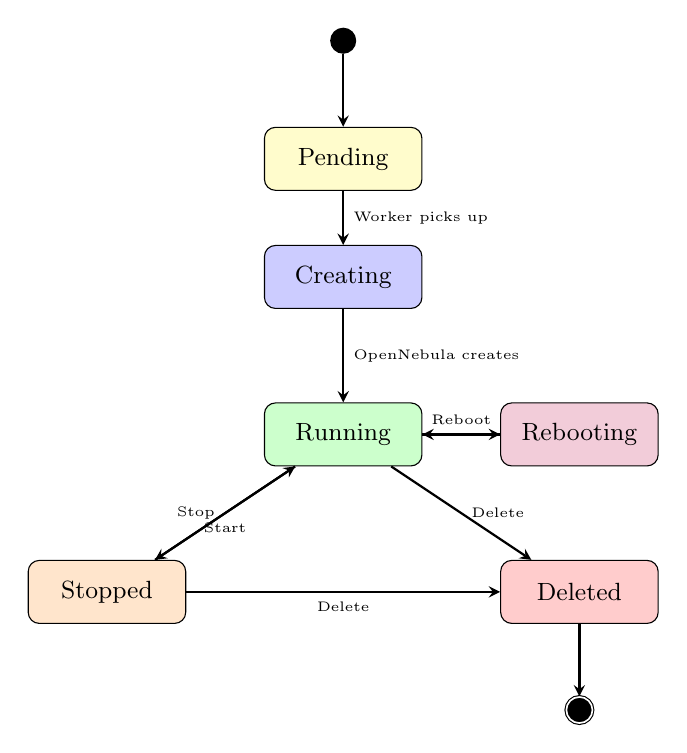
\begin{tikzpicture}[
  state/.style={draw, rounded corners, minimum width=2cm, minimum height=0.8cm, align=center, font=\small},
  decision/.style={draw, diamond, minimum width=1.5cm, minimum height=1cm, align=center, font=\tiny},
  arrow/.style={->, thick, >=stealth}
]
  % States
  \node[circle, fill=black, minimum size=0.3cm] (start) at (0, 0) {};
  \node[state, fill=yellow!20] (pending) at (0, -1.5) {Pending};
  \node[state, fill=blue!20] (creating) at (0, -3) {Creating};
  \node[state, fill=green!20] (running) at (0, -5) {Running};
  \node[state, fill=orange!20] (stopped) at (-3, -7) {Stopped};
  \node[state, fill=red!20] (deleted) at (3, -7) {Deleted};
  \node[state, fill=purple!20] (rebooting) at (3, -5) {Rebooting};
  \node[circle, draw, fill=black, minimum size=0.3cm, double] (end) at (3, -8.5) {};
  
  % Arrows
  \draw[arrow] (start) -- (pending);
  \draw[arrow] (pending) -- node[right, font=\tiny] {Worker picks up} (creating);
  \draw[arrow] (creating) -- node[right, font=\tiny] {OpenNebula creates} (running);
  \draw[arrow] (running) -- node[left, font=\tiny] {Stop} (stopped);
  \draw[arrow] (stopped) -- node[below, font=\tiny] {Start} (running);
  \draw[arrow] (running) -- node[above, font=\tiny] {Reboot} (rebooting);
  \draw[arrow] (rebooting) -- node[right, font=\tiny] {} (running);
  \draw[arrow] (running) -- node[right, font=\tiny] {Delete} (deleted);
  \draw[arrow] (stopped) -- node[below, font=\tiny] {Delete} (deleted);
  \draw[arrow] (deleted) -- (end);
\end{tikzpicture}
\caption{Activity diagram — VM lifecycle}
\label{fig:activity-vm}
\end{figure}

\subsection{Class Diagram — VM Module}

\begin{figure}[H]
\centering
\begin{tikzpicture}[font=\small,
  class/.style={draw, rectangle, minimum width=4cm, align=left}
]
  % VM class
  \node[class, fill=yellow!15] (vmclass) at (0, 0) {
    \textbf{VirtualMachine}\\
    \hline
    - id: UUID\\
    - name: String\\
    - userId: UUID\\
    - templateId: String\\
    - vcpu: Integer\\
    - ram: Integer (MB)\\
    - disk: Integer (GB)\\
    - status: VMStatus\\
    - ipAddress: String\\
    - oneId: Integer\\
    - createdAt: DateTime\\
    \hline
    + create()\\
    + start()\\
    + stop()\\
    + reboot()\\
    + delete()
  };
  
  % VMStatus enum
  \node[class, fill=green!15] (statusenum) at (6, 1) {
    \textbf{<<enum>> VMStatus}\\
    \hline
    PENDING\\
    CREATING\\
    RUNNING\\
    STOPPED\\
    REBOOTING\\
    DELETING\\
    DELETED\\
    ERROR
  };
  
  % VMTemplate
  \node[class, fill=blue!15] (template) at (6, -3.5) {
    \textbf{VMTemplate}\\
    \hline
    - id: String\\
    - name: String\\
    - os: String\\
    - minCpu: Integer\\
    - minRam: Integer\\
    - minDisk: Integer\\
    \hline
    + getTemplates()
  };
  
  % Relations
  \draw[->, thick] (vmclass) -- node[above, font=\tiny] {has} (statusenum);
  \draw[->, thick] (vmclass) -- node[below, font=\tiny] {uses} (template);
\end{tikzpicture}
\caption{Class diagram — VM module}
\label{fig:class-vm}
\end{figure}

\subsection{Architecture Diagram — Worker Communication}

\begin{figure}[H]
\centering
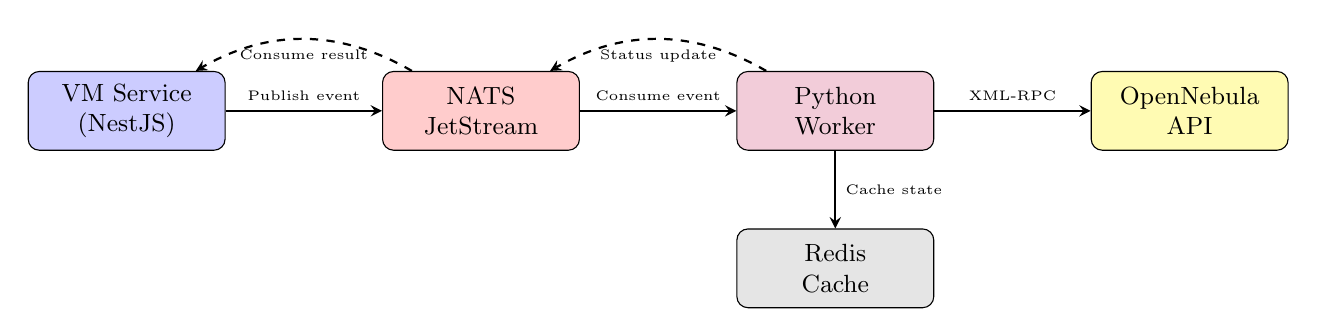
\begin{tikzpicture}[
  box/.style={draw, rounded corners, minimum width=2.5cm, minimum height=1cm, align=center, font=\small},
  arrow/.style={->, thick, >=stealth}
]
  \node[box, fill=blue!20] (vmsvc) at (0, 0) {VM Service\\(NestJS)};
  \node[box, fill=red!20] (nats) at (4.5, 0) {NATS\\JetStream};
  \node[box, fill=purple!20] (worker) at (9, 0) {Python\\Worker};
  \node[box, fill=gray!20] (redis) at (9, -2) {Redis\\Cache};
  \node[box, fill=yellow!30] (one) at (13.5, 0) {OpenNebula\\API};
  
  \draw[arrow] (vmsvc) -- node[above, font=\tiny] {Publish event} (nats);
  \draw[arrow] (nats) -- node[above, font=\tiny] {Consume event} (worker);
  \draw[arrow] (worker) -- node[above, font=\tiny] {XML-RPC} (one);
  \draw[arrow] (worker) -- node[right, font=\tiny] {Cache state} (redis);
  \draw[arrow, dashed] (worker) to[bend right=30] node[below, font=\tiny] {Status update} (nats);
  \draw[arrow, dashed] (nats) to[bend right=30] node[below, font=\tiny] {Consume result} (vmsvc);
\end{tikzpicture}
\caption{Architecture — Worker communication via JetStream}
\label{fig:worker-arch}
\end{figure}

\subsection{Implementation Screenshots}

\begin{figure}[H]
\centering
\fbox{\parbox{0.9\textwidth}{\centering\vspace{3cm}\textit{Insert VM creation form screenshot}\vspace{3cm}}}
\caption{VM creation form}
\label{fig:vm-create-form}
\end{figure}

\begin{figure}[H]
\centering
\fbox{\parbox{0.9\textwidth}{\centering\vspace{3cm}\textit{Insert VM list page screenshot}\vspace{3cm}}}
\caption{VM list page}
\label{fig:vm-list}
\end{figure}

\subsection{Sprint 4 Review}

At the end of Sprint 4:
\begin{itemize}
  \item VM service with full lifecycle operations (create, start, stop, reboot, delete).
  \item Python worker consuming events from NATS JetStream.
  \item Worker communicates with OpenNebula via XML-RPC API.
  \item VM creation form with template selection.
  \item VM list page with status indicators.
  \item OpenNebula virtual networks and storage configured.
  \item End-to-end VM creation working.
\end{itemize}

% ============================================================
\section{Conclusion}

In this chapter, we completed the user management features and the core VM operations. Sprint 3 delivered the admin panel, dashboard layout, and message queue infrastructure. Sprint 4 implemented the central feature of the platform — the ability to create and manage virtual machines through an asynchronous worker that communicates with OpenNebula.

In the next chapter, we will enhance the VM experience with a detailed dashboard, implement the quota system, and build the payment service.

% ============================================================
\chapter{Sprint 3 \& Sprint 4: User Management and VM Operations}

\section{Introduction}

This chapter covers the core features of the platform. Sprint 3 implements user management, the dashboard layout, and NATS JetStream integration. Sprint 4 delivers the central feature — virtual machine lifecycle management through the VM service, Python worker, and OpenNebula integration.

% ============================================================
% SPRINT 3
% ============================================================
\section{Sprint 3: User Management \& Dashboard}

\sprintcard{3}{User Management \& Dashboard}{Implement user CRUD, admin management panel, dashboard layout, and message queue setup.}

\subsection{Sprint Backlog}

\begin{longtable}{|c|p{5cm}|c|c|c|}
\hline
\rowcolor{blue!15}
\textbf{Task ID} & \textbf{Task} & \textbf{Assignee} & \textbf{Est.} & \textbf{Status} \\
\hline
\endhead
T-3.1 & User service CRUD endpoints & DSI & 4h & Done \\
\hline
T-3.2 & Admin user management endpoints & DSI & 3h & Done \\
\hline
T-3.3 & Dashboard layout (sidebar, header) & DSI & 6h & Done \\
\hline
T-3.4 & Profile page (view/edit) & DSI & 4h & Done \\
\hline
T-3.11 & SSH key management (CRUD + UI) & DSI & 5h & Done \\
\hline
T-3.5 & Admin — user list page & DSI & 4h & Done \\
\hline
T-3.6 & NATS JetStream setup & DSI & 4h & Done \\
\hline
T-3.7 & Firewall rules (iptables) & RSI & 6h & Done \\
\hline
T-3.8 & Firewall testing & RSI & 4h & Done \\
\hline
T-3.9 & OpenNebula API access & RSI & 6h & Done \\
\hline
\caption{Sprint 3 backlog}
\label{tab:sprint3-backlog}
\end{longtable}

\subsection{Use Case Diagram — User Management}

\begin{figure}[H]
\centering
\begin{tikzpicture}[
  usecase/.style={draw, ellipse, minimum width=3cm, minimum height=0.8cm, align=center, font=\scriptsize}
]
  % System boundary
  \draw[thick, rounded corners] (0, -6.5) rectangle (6, 0.5);
  \node[font=\small\bfseries] at (3, 0.2) {User Management Module};
  
  % Actors
  \node (user) at (-2, -1.5) {User};
  \node (admin) at (-2, -5) {Admin};
  
  % Use cases
  \node[usecase] (uc1) at (3, -0.5) {View Profile};
  \node[usecase] (uc2) at (3, -1.5) {Edit Profile};
  \node[usecase] (uc3) at (3, -2.5) {Change Password};
  \node[usecase] (uc6) at (3, -3.5) {Manage SSH Keys};
  \node[usecase] (uc4) at (3, -4.5) {View All Users};
  \node[usecase] (uc5) at (3, -5.5) {Delete/Ban User};
  
  % Arrows
  \draw (user) -- (uc1);
  \draw (user) -- (uc2);
  \draw (user) -- (uc3);
  \draw (user) -- (uc6);
  \draw (admin) -- (uc4);
  \draw (admin) -- (uc5);
  
  % Generalization
  \draw[->, dashed] (admin) -- (user);
  
\end{tikzpicture}
\caption{Use case diagram — User management}
\label{fig:uc-user}
\end{figure}

\subsection{Sequence Diagram — Admin Deletes User}

\begin{figure}[H]
\centering
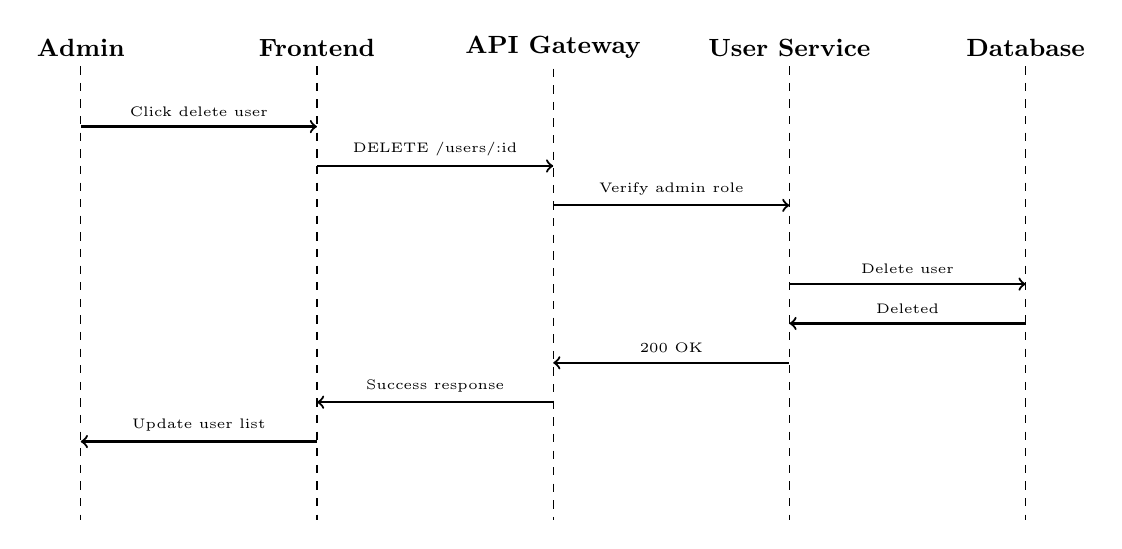
\begin{tikzpicture}[font=\small]
  \node (admin) at (0, 0) {\textbf{Admin}};
  \node (front) at (3, 0) {\textbf{Frontend}};
  \node (gate) at (6, 0) {\textbf{API Gateway}};
  \node (usvc) at (9, 0) {\textbf{User Service}};
  \node (db) at (12, 0) {\textbf{Database}};
  
  \draw[dashed] (admin) -- (0, -6);
  \draw[dashed] (front) -- (3, -6);
  \draw[dashed] (gate) -- (6, -6);
  \draw[dashed] (usvc) -- (9, -6);
  \draw[dashed] (db) -- (12, -6);
  
  \draw[->, thick] (0, -1) -- node[above, font=\tiny] {Click delete user} (3, -1);
  \draw[->, thick] (3, -1.5) -- node[above, font=\tiny] {DELETE /users/:id} (6, -1.5);
  \draw[->, thick] (6, -2) -- node[above, font=\tiny] {Verify admin role} (9, -2);
  \draw[->, thick] (9, -3) -- node[above, font=\tiny] {Delete user} (12, -3);
  \draw[<-, thick] (9, -3.5) -- node[above, font=\tiny] {Deleted} (12, -3.5);
  \draw[<-, thick] (6, -4) -- node[above, font=\tiny] {200 OK} (9, -4);
  \draw[<-, thick] (3, -4.5) -- node[above, font=\tiny] {Success response} (6, -4.5);
  \draw[<-, thick] (0, -5) -- node[above, font=\tiny] {Update user list} (3, -5);
\end{tikzpicture}
\caption{Sequence diagram — Admin deletes user}
\label{fig:seq-delete-user}
\end{figure}

\subsection{Implementation Screenshots}

\begin{figure}[H]
\centering
\fbox{\parbox{0.9\textwidth}{\centering\vspace{3cm}\textit{Insert dashboard layout screenshot}\vspace{3cm}}}
\caption{Dashboard layout with sidebar navigation}
\label{fig:dashboard-layout}
\end{figure}

\begin{figure}[H]
\centering
\fbox{\parbox{0.9\textwidth}{\centering\vspace{3cm}\textit{Insert admin user management screenshot}\vspace{3cm}}}
\caption{Admin — User management page}
\label{fig:admin-users}
\end{figure}

\begin{figure}[H]
\centering
\fbox{\parbox{0.9\textwidth}{\centering\vspace{3cm}\textit{Insert SSH key management page screenshot}\vspace{3cm}}}
\caption{SSH key management — User profile}
\label{fig:ssh-keys}
\end{figure}

\subsection{Sprint 3 Review}

At the end of Sprint 3:
\begin{itemize}
  \item User service with full CRUD operations.
  \item Admin panel for user management.
  \item Dashboard layout with sidebar, header, and responsive design.
  \item Profile page with edit functionality.
  \item SSH key management — users can add, view, and delete SSH public keys.
  \item NATS JetStream configured and tested.
  \item Firewall rules implemented and tested.
  \item OpenNebula XML-RPC API accessible and secured.
\end{itemize}


% ============================================================
% SPRINT 4
% ============================================================
\section{Sprint 4: VM Management \& Worker Service}

\sprintcard{4}{VM Management \& Worker Service}{Implement the core VM lifecycle operations — create, start, stop, reboot, delete — through the web platform with asynchronous processing via the Python worker.}

\subsection{Sprint Backlog}

\begin{longtable}{|c|p{5cm}|c|c|c|}
\hline
\rowcolor{blue!15}
\textbf{Task ID} & \textbf{Task} & \textbf{Assignee} & \textbf{Est.} & \textbf{Status} \\
\hline
\endhead
T-4.1 & VM service — Create VM endpoint & DSI & 5h & Done \\
\hline
T-4.2 & Python worker setup (Redis + NATS) & DSI & 5h & Done \\
\hline
T-4.3 & Worker — Create VM via OpenNebula & DSI & 5h & Done \\
\hline
T-4.4 & Worker — Start/Stop/Reboot ops & DSI & 4h & Done \\
\hline
T-4.5 & Worker — Delete VM operation & DSI & 2h & Done \\
\hline
T-4.6 & VM creation form (frontend) & DSI & 5h & Done \\
\hline
T-4.7 & VM list page (frontend) & DSI & 4h & Done \\
\hline
T-4.8 & OpenNebula API integration testing & RSI & 6h & Done \\
\hline
T-4.9 & VM networking (virtual networks) & RSI & 6h & Done \\
\hline
T-4.10 & Storage + disk images & RSI & 4h & Done \\
\hline
\caption{Sprint 4 backlog}
\label{tab:sprint4-backlog}
\end{longtable}

\subsection{Use Case Diagram — VM Management}

\begin{figure}[H]
\centering
\begin{tikzpicture}[
  usecase/.style={draw, ellipse, minimum width=2.8cm, minimum height=0.8cm, align=center, font=\scriptsize}
]
  % System boundary
  \draw[thick, rounded corners] (0, -7) rectangle (6.5, 0.5);
  \node[font=\small\bfseries] at (3.25, 0.2) {VM Management Module};
  
  % Actors
  \node (user) at (-2, -2) {User};
  \node (admin) at (9, -3) {Admin};
  
  % Use cases
  \node[usecase] (uc1) at (3.25, -0.5) {Create VM};
  \node[usecase] (uc2) at (3.25, -1.5) {Start VM};
  \node[usecase] (uc3) at (3.25, -2.5) {Stop VM};
  \node[usecase] (uc4) at (3.25, -3.5) {Reboot VM};
  \node[usecase] (uc5) at (3.25, -4.5) {Delete VM};
  \node[usecase] (uc6) at (3.25, -5.5) {View VM List};
  \node[usecase] (uc7) at (3.25, -6.5) {View VM Details};
  
  % Arrows
  \draw (user) -- (uc1);
  \draw (user) -- (uc2);
  \draw (user) -- (uc3);
  \draw (user) -- (uc4);
  \draw (user) -- (uc5);
  \draw (user) -- (uc6);
  \draw (user) -- (uc7);
  
  \draw (admin) -- (uc1);
  \draw (admin) -- (uc5);
  \draw (admin) -- (uc6);
  
\end{tikzpicture}
\caption{Use case diagram — VM management}
\label{fig:uc-vm}
\end{figure}

\subsection{Sequence Diagram — VM Creation (End-to-End)}

\begin{figure}[H]
\centering
\begin{tikzpicture}[font=\scriptsize]
  % Lifelines
  \node (user) at (0, 0) {\textbf{User}};
  \node (front) at (2, 0) {\textbf{Frontend}};
  \node (gate) at (4, 0) {\textbf{Gateway}};
  \node (vmsvc) at (6, 0) {\textbf{VM Service}};
  \node (nats) at (8, 0) {\textbf{JetStream}};
  \node (worker) at (10, 0) {\textbf{Worker}};
  \node (one) at (12.5, 0) {\textbf{OpenNebula}};
  
  \draw[dashed] (user) -- (0, -11);
  \draw[dashed] (front) -- (2, -11);
  \draw[dashed] (gate) -- (4, -11);
  \draw[dashed] (vmsvc) -- (6, -11);
  \draw[dashed] (nats) -- (8, -11);
  \draw[dashed] (worker) -- (10, -11);
  \draw[dashed] (one) -- (12.5, -11);
  
  % Messages
  \draw[->, thick] (0, -0.8) -- node[above] {Fill VM form} (2, -0.8);
  \draw[->, thick] (2, -1.5) -- node[above] {POST /vms} (4, -1.5);
  \draw[->, thick] (4, -2.2) -- node[above] {Forward} (6, -2.2);
  \draw[->, thick] (6, -2.7) -- node[right] {Check quota};
  \draw[->, thick] (6, -3.5) -- node[above] {Save VM (pending)} (6, -3.5);
  \draw[->, thick] (6, -4.2) -- node[above] {Publish event} (8, -4.2);
  \draw[<-, thick] (4, -4.9) -- node[above] {202 Accepted} (6, -4.9);
  \draw[<-, thick] (2, -5.3) -- node[above] {VM creating...} (4, -5.3);
  \draw[->, thick] (8, -6) -- node[above] {Consume event} (10, -6);
  \draw[->, thick] (10, -6.7) -- node[above] {Create VM} (12.5, -6.7);
  \draw[<-, thick] (10, -7.4) -- node[above] {VM ID + IP} (12.5, -7.4);
  \draw[->, thick] (10, -8.1) -- node[above] {Publish result} (8, -8.1);
  \draw[->, thick] (6, -8.8) -- node[above] {Update status} (6, -8.8);
  \draw[->, thick] (6, -9) -- node[right] {VM → running};
  \draw[<-, thick] (2, -9.7) -- node[above] {Status update} (6, -9.7);
  \draw[<-, thick] (0, -10.3) -- node[above] {VM ready!} (2, -10.3);
\end{tikzpicture}
\caption{Sequence diagram — VM creation (end-to-end)}
\label{fig:seq-vm-create}
\end{figure}

\subsection{Activity Diagram — VM Lifecycle}

\begin{figure}[H]
\centering
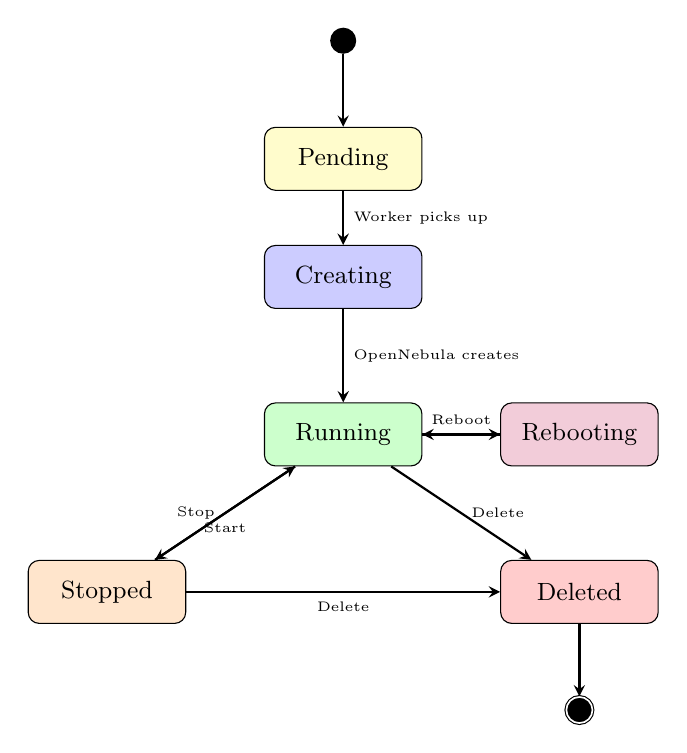
\begin{tikzpicture}[
  state/.style={draw, rounded corners, minimum width=2cm, minimum height=0.8cm, align=center, font=\small},
  decision/.style={draw, diamond, minimum width=1.5cm, minimum height=1cm, align=center, font=\tiny},
  arrow/.style={->, thick, >=stealth}
]
  % States
  \node[circle, fill=black, minimum size=0.3cm] (start) at (0, 0) {};
  \node[state, fill=yellow!20] (pending) at (0, -1.5) {Pending};
  \node[state, fill=blue!20] (creating) at (0, -3) {Creating};
  \node[state, fill=green!20] (running) at (0, -5) {Running};
  \node[state, fill=orange!20] (stopped) at (-3, -7) {Stopped};
  \node[state, fill=red!20] (deleted) at (3, -7) {Deleted};
  \node[state, fill=purple!20] (rebooting) at (3, -5) {Rebooting};
  \node[circle, draw, fill=black, minimum size=0.3cm, double] (end) at (3, -8.5) {};
  
  % Arrows
  \draw[arrow] (start) -- (pending);
  \draw[arrow] (pending) -- node[right, font=\tiny] {Worker picks up} (creating);
  \draw[arrow] (creating) -- node[right, font=\tiny] {OpenNebula creates} (running);
  \draw[arrow] (running) -- node[left, font=\tiny] {Stop} (stopped);
  \draw[arrow] (stopped) -- node[below, font=\tiny] {Start} (running);
  \draw[arrow] (running) -- node[above, font=\tiny] {Reboot} (rebooting);
  \draw[arrow] (rebooting) -- node[right, font=\tiny] {} (running);
  \draw[arrow] (running) -- node[right, font=\tiny] {Delete} (deleted);
  \draw[arrow] (stopped) -- node[below, font=\tiny] {Delete} (deleted);
  \draw[arrow] (deleted) -- (end);
\end{tikzpicture}
\caption{Activity diagram — VM lifecycle}
\label{fig:activity-vm}
\end{figure}

\subsection{Class Diagram — VM Module}

\begin{figure}[H]
\centering
\begin{tikzpicture}[font=\small,
  class/.style={draw, rectangle, minimum width=4cm, align=left}
]
  % VM class
  \node[class, fill=yellow!15] (vmclass) at (0, 0) {
    \textbf{VirtualMachine}\\
    \hline
    - id: UUID\\
    - name: String\\
    - userId: UUID\\
    - templateId: String\\
    - vcpu: Integer\\
    - ram: Integer (MB)\\
    - disk: Integer (GB)\\
    - status: VMStatus\\
    - ipAddress: String\\
    - oneId: Integer\\
    - createdAt: DateTime\\
    \hline
    + create()\\
    + start()\\
    + stop()\\
    + reboot()\\
    + delete()
  };
  
  % VMStatus enum
  \node[class, fill=green!15] (statusenum) at (6, 1) {
    \textbf{<<enum>> VMStatus}\\
    \hline
    PENDING\\
    CREATING\\
    RUNNING\\
    STOPPED\\
    REBOOTING\\
    DELETING\\
    DELETED\\
    ERROR
  };
  
  % VMTemplate
  \node[class, fill=blue!15] (template) at (6, -3.5) {
    \textbf{VMTemplate}\\
    \hline
    - id: String\\
    - name: String\\
    - os: String\\
    - minCpu: Integer\\
    - minRam: Integer\\
    - minDisk: Integer\\
    \hline
    + getTemplates()
  };
  
  % Relations
  \draw[->, thick] (vmclass) -- node[above, font=\tiny] {has} (statusenum);
  \draw[->, thick] (vmclass) -- node[below, font=\tiny] {uses} (template);
\end{tikzpicture}
\caption{Class diagram — VM module}
\label{fig:class-vm}
\end{figure}

\subsection{Architecture Diagram — Worker Communication}

\begin{figure}[H]
\centering
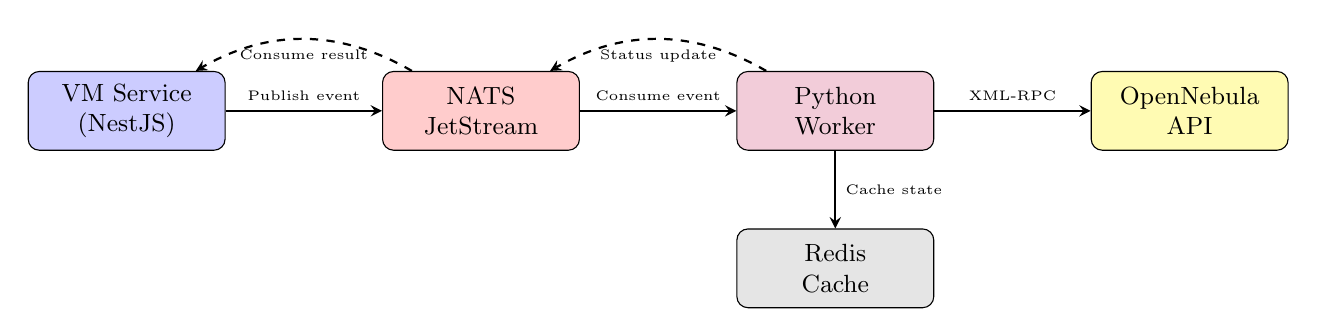
\begin{tikzpicture}[
  box/.style={draw, rounded corners, minimum width=2.5cm, minimum height=1cm, align=center, font=\small},
  arrow/.style={->, thick, >=stealth}
]
  \node[box, fill=blue!20] (vmsvc) at (0, 0) {VM Service\\(NestJS)};
  \node[box, fill=red!20] (nats) at (4.5, 0) {NATS\\JetStream};
  \node[box, fill=purple!20] (worker) at (9, 0) {Python\\Worker};
  \node[box, fill=gray!20] (redis) at (9, -2) {Redis\\Cache};
  \node[box, fill=yellow!30] (one) at (13.5, 0) {OpenNebula\\API};
  
  \draw[arrow] (vmsvc) -- node[above, font=\tiny] {Publish event} (nats);
  \draw[arrow] (nats) -- node[above, font=\tiny] {Consume event} (worker);
  \draw[arrow] (worker) -- node[above, font=\tiny] {XML-RPC} (one);
  \draw[arrow] (worker) -- node[right, font=\tiny] {Cache state} (redis);
  \draw[arrow, dashed] (worker) to[bend right=30] node[below, font=\tiny] {Status update} (nats);
  \draw[arrow, dashed] (nats) to[bend right=30] node[below, font=\tiny] {Consume result} (vmsvc);
\end{tikzpicture}
\caption{Architecture — Worker communication via JetStream}
\label{fig:worker-arch}
\end{figure}

\subsection{Implementation Screenshots}

\begin{figure}[H]
\centering
\fbox{\parbox{0.9\textwidth}{\centering\vspace{3cm}\textit{Insert VM creation form screenshot}\vspace{3cm}}}
\caption{VM creation form}
\label{fig:vm-create-form}
\end{figure}

\begin{figure}[H]
\centering
\fbox{\parbox{0.9\textwidth}{\centering\vspace{3cm}\textit{Insert VM list page screenshot}\vspace{3cm}}}
\caption{VM list page}
\label{fig:vm-list}
\end{figure}

\subsection{Sprint 4 Review}

At the end of Sprint 4:
\begin{itemize}
  \item VM service with full lifecycle operations (create, start, stop, reboot, delete).
  \item Python worker consuming events from NATS JetStream.
  \item Worker communicates with OpenNebula via XML-RPC API.
  \item VM creation form with template selection.
  \item VM list page with status indicators.
  \item OpenNebula virtual networks and storage configured.
  \item End-to-end VM creation working.
\end{itemize}

% ============================================================
\section{Conclusion}

In this chapter, we completed the user management features and the core VM operations. Sprint 3 delivered the admin panel, dashboard layout, and message queue infrastructure. Sprint 4 implemented the central feature of the platform — the ability to create and manage virtual machines through an asynchronous worker that communicates with OpenNebula.

In the next chapter, we will enhance the VM experience with a detailed dashboard, implement the quota system, and build the payment service.

% ============================================================
\chapter{Sprint 3 \& Sprint 4: User Management and VM Operations}

\section{Introduction}

This chapter covers the core features of the platform. Sprint 3 implements user management, the dashboard layout, and NATS JetStream integration. Sprint 4 delivers the central feature — virtual machine lifecycle management through the VM service, Python worker, and OpenNebula integration.

% ============================================================
% SPRINT 3
% ============================================================
\section{Sprint 3: User Management \& Dashboard}

\sprintcard{3}{User Management \& Dashboard}{Implement user CRUD, admin management panel, dashboard layout, and message queue setup.}

\subsection{Sprint Backlog}

\begin{longtable}{|c|p{5cm}|c|c|c|}
\hline
\rowcolor{blue!15}
\textbf{Task ID} & \textbf{Task} & \textbf{Assignee} & \textbf{Est.} & \textbf{Status} \\
\hline
\endhead
T-3.1 & User service CRUD endpoints & DSI & 4h & Done \\
\hline
T-3.2 & Admin user management endpoints & DSI & 3h & Done \\
\hline
T-3.3 & Dashboard layout (sidebar, header) & DSI & 6h & Done \\
\hline
T-3.4 & Profile page (view/edit) & DSI & 4h & Done \\
\hline
T-3.11 & SSH key management (CRUD + UI) & DSI & 5h & Done \\
\hline
T-3.5 & Admin — user list page & DSI & 4h & Done \\
\hline
T-3.6 & NATS JetStream setup & DSI & 4h & Done \\
\hline
T-3.7 & Firewall rules (iptables) & RSI & 6h & Done \\
\hline
T-3.8 & Firewall testing & RSI & 4h & Done \\
\hline
T-3.9 & OpenNebula API access & RSI & 6h & Done \\
\hline
\caption{Sprint 3 backlog}
\label{tab:sprint3-backlog}
\end{longtable}

\subsection{Use Case Diagram — User Management}

\begin{figure}[H]
\centering
\begin{tikzpicture}[
  usecase/.style={draw, ellipse, minimum width=3cm, minimum height=0.8cm, align=center, font=\scriptsize}
]
  % System boundary
  \draw[thick, rounded corners] (0, -6.5) rectangle (6, 0.5);
  \node[font=\small\bfseries] at (3, 0.2) {User Management Module};
  
  % Actors
  \node (user) at (-2, -1.5) {User};
  \node (admin) at (-2, -5) {Admin};
  
  % Use cases
  \node[usecase] (uc1) at (3, -0.5) {View Profile};
  \node[usecase] (uc2) at (3, -1.5) {Edit Profile};
  \node[usecase] (uc3) at (3, -2.5) {Change Password};
  \node[usecase] (uc6) at (3, -3.5) {Manage SSH Keys};
  \node[usecase] (uc4) at (3, -4.5) {View All Users};
  \node[usecase] (uc5) at (3, -5.5) {Delete/Ban User};
  
  % Arrows
  \draw (user) -- (uc1);
  \draw (user) -- (uc2);
  \draw (user) -- (uc3);
  \draw (user) -- (uc6);
  \draw (admin) -- (uc4);
  \draw (admin) -- (uc5);
  
  % Generalization
  \draw[->, dashed] (admin) -- (user);
  
\end{tikzpicture}
\caption{Use case diagram — User management}
\label{fig:uc-user}
\end{figure}

\subsection{Sequence Diagram — Admin Deletes User}

\begin{figure}[H]
\centering
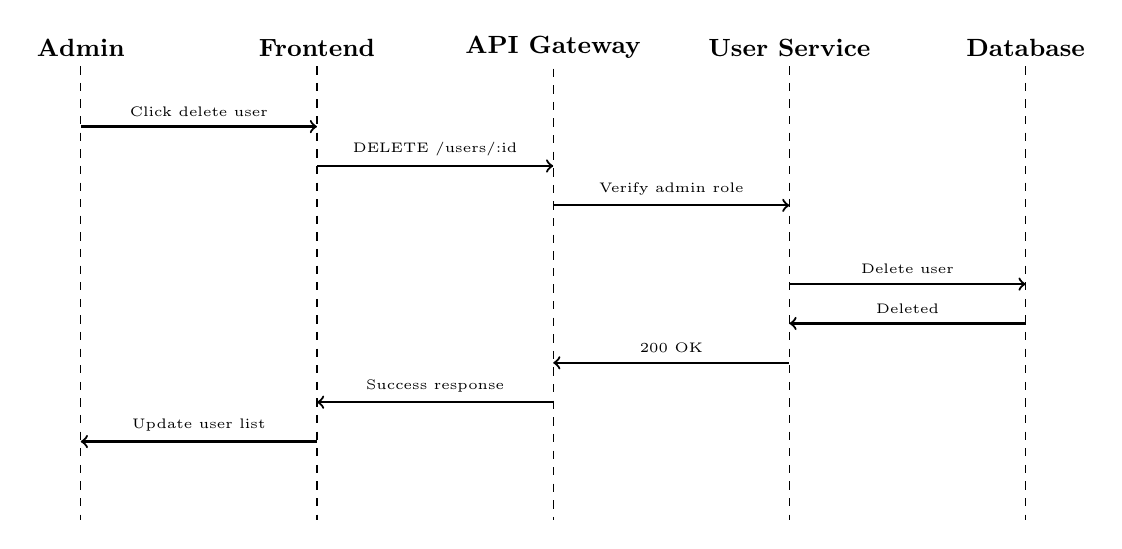
\begin{tikzpicture}[font=\small]
  \node (admin) at (0, 0) {\textbf{Admin}};
  \node (front) at (3, 0) {\textbf{Frontend}};
  \node (gate) at (6, 0) {\textbf{API Gateway}};
  \node (usvc) at (9, 0) {\textbf{User Service}};
  \node (db) at (12, 0) {\textbf{Database}};
  
  \draw[dashed] (admin) -- (0, -6);
  \draw[dashed] (front) -- (3, -6);
  \draw[dashed] (gate) -- (6, -6);
  \draw[dashed] (usvc) -- (9, -6);
  \draw[dashed] (db) -- (12, -6);
  
  \draw[->, thick] (0, -1) -- node[above, font=\tiny] {Click delete user} (3, -1);
  \draw[->, thick] (3, -1.5) -- node[above, font=\tiny] {DELETE /users/:id} (6, -1.5);
  \draw[->, thick] (6, -2) -- node[above, font=\tiny] {Verify admin role} (9, -2);
  \draw[->, thick] (9, -3) -- node[above, font=\tiny] {Delete user} (12, -3);
  \draw[<-, thick] (9, -3.5) -- node[above, font=\tiny] {Deleted} (12, -3.5);
  \draw[<-, thick] (6, -4) -- node[above, font=\tiny] {200 OK} (9, -4);
  \draw[<-, thick] (3, -4.5) -- node[above, font=\tiny] {Success response} (6, -4.5);
  \draw[<-, thick] (0, -5) -- node[above, font=\tiny] {Update user list} (3, -5);
\end{tikzpicture}
\caption{Sequence diagram — Admin deletes user}
\label{fig:seq-delete-user}
\end{figure}

\subsection{Implementation Screenshots}

\begin{figure}[H]
\centering
\fbox{\parbox{0.9\textwidth}{\centering\vspace{3cm}\textit{Insert dashboard layout screenshot}\vspace{3cm}}}
\caption{Dashboard layout with sidebar navigation}
\label{fig:dashboard-layout}
\end{figure}

\begin{figure}[H]
\centering
\fbox{\parbox{0.9\textwidth}{\centering\vspace{3cm}\textit{Insert admin user management screenshot}\vspace{3cm}}}
\caption{Admin — User management page}
\label{fig:admin-users}
\end{figure}

\begin{figure}[H]
\centering
\fbox{\parbox{0.9\textwidth}{\centering\vspace{3cm}\textit{Insert SSH key management page screenshot}\vspace{3cm}}}
\caption{SSH key management — User profile}
\label{fig:ssh-keys}
\end{figure}

\subsection{Sprint 3 Review}

At the end of Sprint 3:
\begin{itemize}
  \item User service with full CRUD operations.
  \item Admin panel for user management.
  \item Dashboard layout with sidebar, header, and responsive design.
  \item Profile page with edit functionality.
  \item SSH key management — users can add, view, and delete SSH public keys.
  \item NATS JetStream configured and tested.
  \item Firewall rules implemented and tested.
  \item OpenNebula XML-RPC API accessible and secured.
\end{itemize}


% ============================================================
% SPRINT 4
% ============================================================
\section{Sprint 4: VM Management \& Worker Service}

\sprintcard{4}{VM Management \& Worker Service}{Implement the core VM lifecycle operations — create, start, stop, reboot, delete — through the web platform with asynchronous processing via the Python worker.}

\subsection{Sprint Backlog}

\begin{longtable}{|c|p{5cm}|c|c|c|}
\hline
\rowcolor{blue!15}
\textbf{Task ID} & \textbf{Task} & \textbf{Assignee} & \textbf{Est.} & \textbf{Status} \\
\hline
\endhead
T-4.1 & VM service — Create VM endpoint & DSI & 5h & Done \\
\hline
T-4.2 & Python worker setup (Redis + NATS) & DSI & 5h & Done \\
\hline
T-4.3 & Worker — Create VM via OpenNebula & DSI & 5h & Done \\
\hline
T-4.4 & Worker — Start/Stop/Reboot ops & DSI & 4h & Done \\
\hline
T-4.5 & Worker — Delete VM operation & DSI & 2h & Done \\
\hline
T-4.6 & VM creation form (frontend) & DSI & 5h & Done \\
\hline
T-4.7 & VM list page (frontend) & DSI & 4h & Done \\
\hline
T-4.8 & OpenNebula API integration testing & RSI & 6h & Done \\
\hline
T-4.9 & VM networking (virtual networks) & RSI & 6h & Done \\
\hline
T-4.10 & Storage + disk images & RSI & 4h & Done \\
\hline
\caption{Sprint 4 backlog}
\label{tab:sprint4-backlog}
\end{longtable}

\subsection{Use Case Diagram — VM Management}

\begin{figure}[H]
\centering
\begin{tikzpicture}[
  usecase/.style={draw, ellipse, minimum width=2.8cm, minimum height=0.8cm, align=center, font=\scriptsize}
]
  % System boundary
  \draw[thick, rounded corners] (0, -7) rectangle (6.5, 0.5);
  \node[font=\small\bfseries] at (3.25, 0.2) {VM Management Module};
  
  % Actors
  \node (user) at (-2, -2) {User};
  \node (admin) at (9, -3) {Admin};
  
  % Use cases
  \node[usecase] (uc1) at (3.25, -0.5) {Create VM};
  \node[usecase] (uc2) at (3.25, -1.5) {Start VM};
  \node[usecase] (uc3) at (3.25, -2.5) {Stop VM};
  \node[usecase] (uc4) at (3.25, -3.5) {Reboot VM};
  \node[usecase] (uc5) at (3.25, -4.5) {Delete VM};
  \node[usecase] (uc6) at (3.25, -5.5) {View VM List};
  \node[usecase] (uc7) at (3.25, -6.5) {View VM Details};
  
  % Arrows
  \draw (user) -- (uc1);
  \draw (user) -- (uc2);
  \draw (user) -- (uc3);
  \draw (user) -- (uc4);
  \draw (user) -- (uc5);
  \draw (user) -- (uc6);
  \draw (user) -- (uc7);
  
  \draw (admin) -- (uc1);
  \draw (admin) -- (uc5);
  \draw (admin) -- (uc6);
  
\end{tikzpicture}
\caption{Use case diagram — VM management}
\label{fig:uc-vm}
\end{figure}

\subsection{Sequence Diagram — VM Creation (End-to-End)}

\begin{figure}[H]
\centering
\begin{tikzpicture}[font=\scriptsize]
  % Lifelines
  \node (user) at (0, 0) {\textbf{User}};
  \node (front) at (2, 0) {\textbf{Frontend}};
  \node (gate) at (4, 0) {\textbf{Gateway}};
  \node (vmsvc) at (6, 0) {\textbf{VM Service}};
  \node (nats) at (8, 0) {\textbf{JetStream}};
  \node (worker) at (10, 0) {\textbf{Worker}};
  \node (one) at (12.5, 0) {\textbf{OpenNebula}};
  
  \draw[dashed] (user) -- (0, -11);
  \draw[dashed] (front) -- (2, -11);
  \draw[dashed] (gate) -- (4, -11);
  \draw[dashed] (vmsvc) -- (6, -11);
  \draw[dashed] (nats) -- (8, -11);
  \draw[dashed] (worker) -- (10, -11);
  \draw[dashed] (one) -- (12.5, -11);
  
  % Messages
  \draw[->, thick] (0, -0.8) -- node[above] {Fill VM form} (2, -0.8);
  \draw[->, thick] (2, -1.5) -- node[above] {POST /vms} (4, -1.5);
  \draw[->, thick] (4, -2.2) -- node[above] {Forward} (6, -2.2);
  \draw[->, thick] (6, -2.7) -- node[right] {Check quota};
  \draw[->, thick] (6, -3.5) -- node[above] {Save VM (pending)} (6, -3.5);
  \draw[->, thick] (6, -4.2) -- node[above] {Publish event} (8, -4.2);
  \draw[<-, thick] (4, -4.9) -- node[above] {202 Accepted} (6, -4.9);
  \draw[<-, thick] (2, -5.3) -- node[above] {VM creating...} (4, -5.3);
  \draw[->, thick] (8, -6) -- node[above] {Consume event} (10, -6);
  \draw[->, thick] (10, -6.7) -- node[above] {Create VM} (12.5, -6.7);
  \draw[<-, thick] (10, -7.4) -- node[above] {VM ID + IP} (12.5, -7.4);
  \draw[->, thick] (10, -8.1) -- node[above] {Publish result} (8, -8.1);
  \draw[->, thick] (6, -8.8) -- node[above] {Update status} (6, -8.8);
  \draw[->, thick] (6, -9) -- node[right] {VM → running};
  \draw[<-, thick] (2, -9.7) -- node[above] {Status update} (6, -9.7);
  \draw[<-, thick] (0, -10.3) -- node[above] {VM ready!} (2, -10.3);
\end{tikzpicture}
\caption{Sequence diagram — VM creation (end-to-end)}
\label{fig:seq-vm-create}
\end{figure}

\subsection{Activity Diagram — VM Lifecycle}

\begin{figure}[H]
\centering
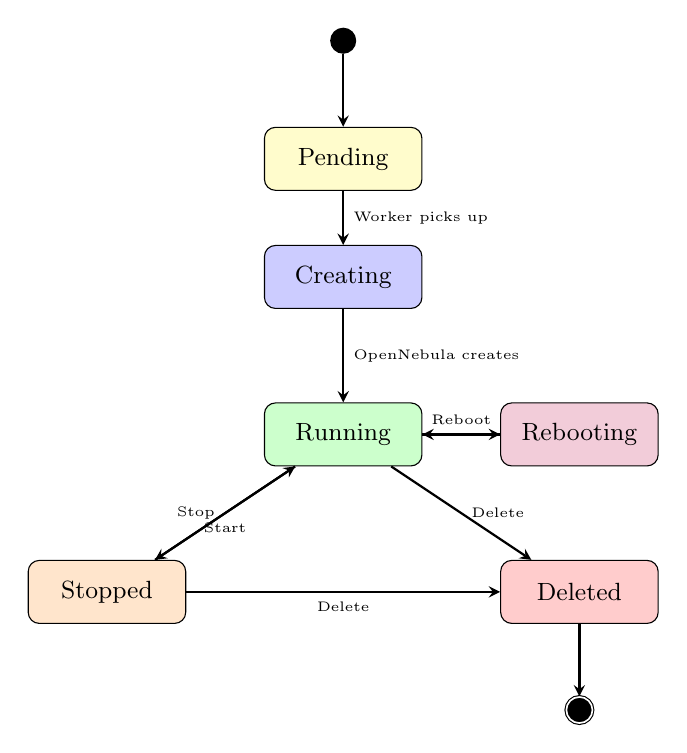
\begin{tikzpicture}[
  state/.style={draw, rounded corners, minimum width=2cm, minimum height=0.8cm, align=center, font=\small},
  decision/.style={draw, diamond, minimum width=1.5cm, minimum height=1cm, align=center, font=\tiny},
  arrow/.style={->, thick, >=stealth}
]
  % States
  \node[circle, fill=black, minimum size=0.3cm] (start) at (0, 0) {};
  \node[state, fill=yellow!20] (pending) at (0, -1.5) {Pending};
  \node[state, fill=blue!20] (creating) at (0, -3) {Creating};
  \node[state, fill=green!20] (running) at (0, -5) {Running};
  \node[state, fill=orange!20] (stopped) at (-3, -7) {Stopped};
  \node[state, fill=red!20] (deleted) at (3, -7) {Deleted};
  \node[state, fill=purple!20] (rebooting) at (3, -5) {Rebooting};
  \node[circle, draw, fill=black, minimum size=0.3cm, double] (end) at (3, -8.5) {};
  
  % Arrows
  \draw[arrow] (start) -- (pending);
  \draw[arrow] (pending) -- node[right, font=\tiny] {Worker picks up} (creating);
  \draw[arrow] (creating) -- node[right, font=\tiny] {OpenNebula creates} (running);
  \draw[arrow] (running) -- node[left, font=\tiny] {Stop} (stopped);
  \draw[arrow] (stopped) -- node[below, font=\tiny] {Start} (running);
  \draw[arrow] (running) -- node[above, font=\tiny] {Reboot} (rebooting);
  \draw[arrow] (rebooting) -- node[right, font=\tiny] {} (running);
  \draw[arrow] (running) -- node[right, font=\tiny] {Delete} (deleted);
  \draw[arrow] (stopped) -- node[below, font=\tiny] {Delete} (deleted);
  \draw[arrow] (deleted) -- (end);
\end{tikzpicture}
\caption{Activity diagram — VM lifecycle}
\label{fig:activity-vm}
\end{figure}

\subsection{Class Diagram — VM Module}

\begin{figure}[H]
\centering
\begin{tikzpicture}[font=\small,
  class/.style={draw, rectangle, minimum width=4cm, align=left}
]
  % VM class
  \node[class, fill=yellow!15] (vmclass) at (0, 0) {
    \textbf{VirtualMachine}\\
    \hline
    - id: UUID\\
    - name: String\\
    - userId: UUID\\
    - templateId: String\\
    - vcpu: Integer\\
    - ram: Integer (MB)\\
    - disk: Integer (GB)\\
    - status: VMStatus\\
    - ipAddress: String\\
    - oneId: Integer\\
    - createdAt: DateTime\\
    \hline
    + create()\\
    + start()\\
    + stop()\\
    + reboot()\\
    + delete()
  };
  
  % VMStatus enum
  \node[class, fill=green!15] (statusenum) at (6, 1) {
    \textbf{<<enum>> VMStatus}\\
    \hline
    PENDING\\
    CREATING\\
    RUNNING\\
    STOPPED\\
    REBOOTING\\
    DELETING\\
    DELETED\\
    ERROR
  };
  
  % VMTemplate
  \node[class, fill=blue!15] (template) at (6, -3.5) {
    \textbf{VMTemplate}\\
    \hline
    - id: String\\
    - name: String\\
    - os: String\\
    - minCpu: Integer\\
    - minRam: Integer\\
    - minDisk: Integer\\
    \hline
    + getTemplates()
  };
  
  % Relations
  \draw[->, thick] (vmclass) -- node[above, font=\tiny] {has} (statusenum);
  \draw[->, thick] (vmclass) -- node[below, font=\tiny] {uses} (template);
\end{tikzpicture}
\caption{Class diagram — VM module}
\label{fig:class-vm}
\end{figure}

\subsection{Architecture Diagram — Worker Communication}

\begin{figure}[H]
\centering
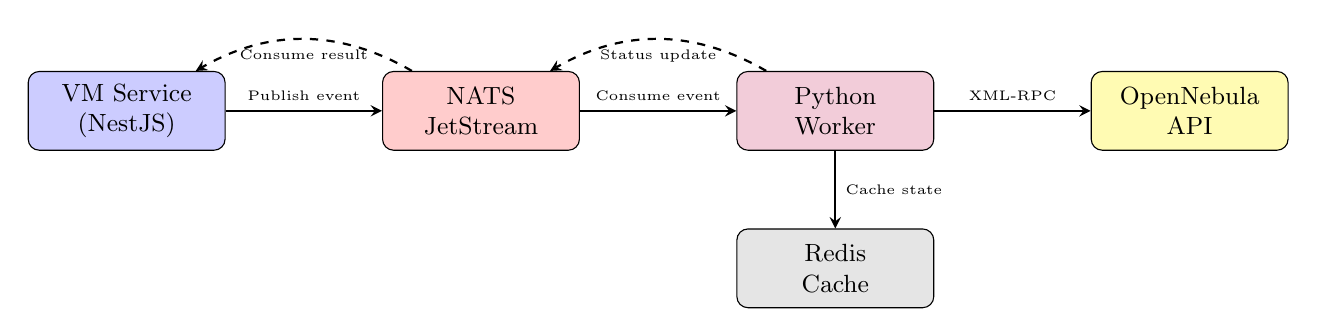
\begin{tikzpicture}[
  box/.style={draw, rounded corners, minimum width=2.5cm, minimum height=1cm, align=center, font=\small},
  arrow/.style={->, thick, >=stealth}
]
  \node[box, fill=blue!20] (vmsvc) at (0, 0) {VM Service\\(NestJS)};
  \node[box, fill=red!20] (nats) at (4.5, 0) {NATS\\JetStream};
  \node[box, fill=purple!20] (worker) at (9, 0) {Python\\Worker};
  \node[box, fill=gray!20] (redis) at (9, -2) {Redis\\Cache};
  \node[box, fill=yellow!30] (one) at (13.5, 0) {OpenNebula\\API};
  
  \draw[arrow] (vmsvc) -- node[above, font=\tiny] {Publish event} (nats);
  \draw[arrow] (nats) -- node[above, font=\tiny] {Consume event} (worker);
  \draw[arrow] (worker) -- node[above, font=\tiny] {XML-RPC} (one);
  \draw[arrow] (worker) -- node[right, font=\tiny] {Cache state} (redis);
  \draw[arrow, dashed] (worker) to[bend right=30] node[below, font=\tiny] {Status update} (nats);
  \draw[arrow, dashed] (nats) to[bend right=30] node[below, font=\tiny] {Consume result} (vmsvc);
\end{tikzpicture}
\caption{Architecture — Worker communication via JetStream}
\label{fig:worker-arch}
\end{figure}

\subsection{Implementation Screenshots}

\begin{figure}[H]
\centering
\fbox{\parbox{0.9\textwidth}{\centering\vspace{3cm}\textit{Insert VM creation form screenshot}\vspace{3cm}}}
\caption{VM creation form}
\label{fig:vm-create-form}
\end{figure}

\begin{figure}[H]
\centering
\fbox{\parbox{0.9\textwidth}{\centering\vspace{3cm}\textit{Insert VM list page screenshot}\vspace{3cm}}}
\caption{VM list page}
\label{fig:vm-list}
\end{figure}

\subsection{Sprint 4 Review}

At the end of Sprint 4:
\begin{itemize}
  \item VM service with full lifecycle operations (create, start, stop, reboot, delete).
  \item Python worker consuming events from NATS JetStream.
  \item Worker communicates with OpenNebula via XML-RPC API.
  \item VM creation form with template selection.
  \item VM list page with status indicators.
  \item OpenNebula virtual networks and storage configured.
  \item End-to-end VM creation working.
\end{itemize}

% ============================================================
\section{Conclusion}

In this chapter, we completed the user management features and the core VM operations. Sprint 3 delivered the admin panel, dashboard layout, and message queue infrastructure. Sprint 4 implemented the central feature of the platform — the ability to create and manage virtual machines through an asynchronous worker that communicates with OpenNebula.

In the next chapter, we will enhance the VM experience with a detailed dashboard, implement the quota system, and build the payment service.
